\chapter{Type Classes and Type Inference}
\begin{figure}[htbp]
   \centering
   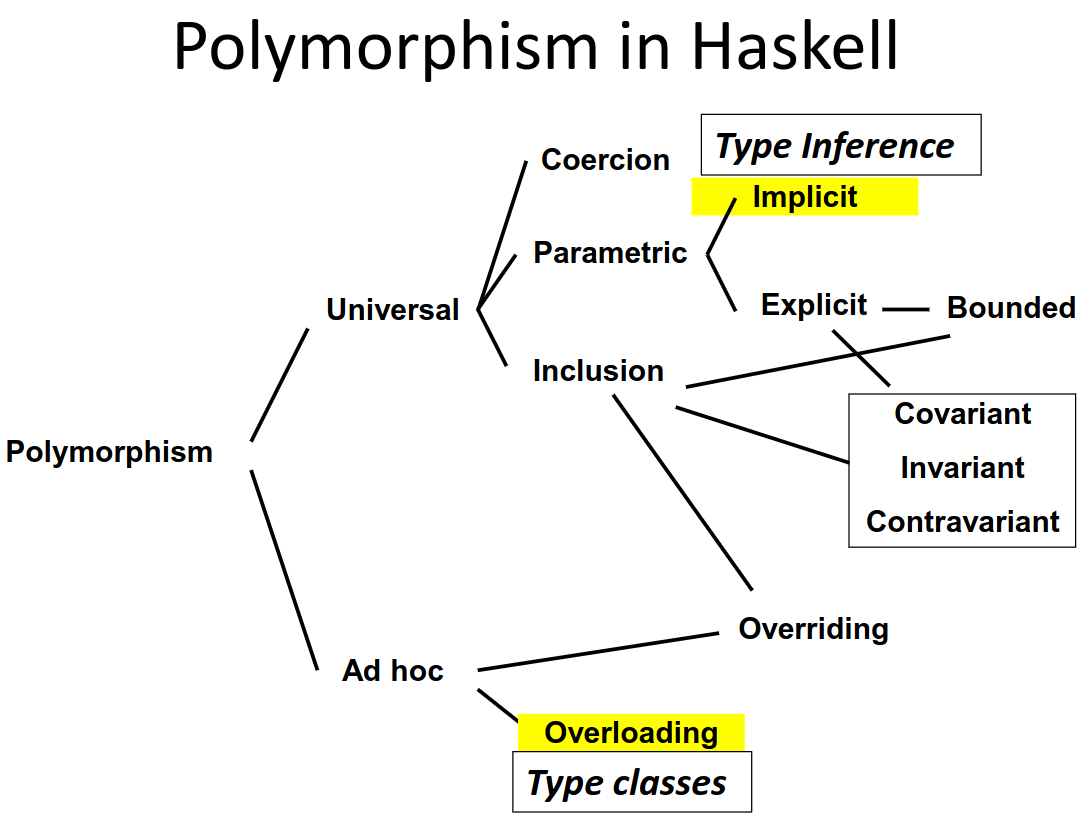
\includegraphics{images/haskell_polymorphism.png}
   \caption{Haskell Polymorphism Recap}
   \label{fig:haskell_polymorphism}
\end{figure}

\section{Overloading}
Haskell allows \textbf{overloading} even of \textbf{primitive types}:
the code to be executed is determined by the type of the arguments,
leading to have \textit{early binding} in \textit{statically} typed languages
or \textit{late binding} in \textit{dynamically} typed languages.

In Haskell we can write the following, but what is the type? May be float, int, double, etc.
\begin{lstlisting}
   sqr x = x * x
\end{lstlisting}

\note{
   \tiny
   Actually in Haskell, we have \ul{type classes}
   \texttt{sqr :: Num a => a -> a}
}

When considering overloading besides arithmetic, we find that some functions are \textbf{fully polymorphic}:
\begin{lstlisting}
   length :: [w] -> Int
\end{lstlisting}

While others not so much;
for example, \textit{membership} works only for types that support equality,
while \textit{sorting} works only for types which support \textit{ordering}. Hence we must try to write the signature in a way that reflects this, not accepting any type as if such functions were fully polymorphic.
\begin{lstlisting}
   member :: [w] -> w -> Bool
   sort :: [w] -> [w]
\end{lstlisting}

\subsection{Possible Overloading solutions}
\begin{lstlisting}
   --- This may be Int -> Int or Float -> Float
   square x = x * x

   --- This is a mess
   squares (x,y,z) = (square x, square y, square z)
\end{lstlisting}
An idea might be to implicitly define function for each possible combination of types, but this is typically not feasible.
In the above example \lstinline|squares| generates 8 possible functions, and this is just for a 3-tuple.
The growth is exponential, so this is not a viable solution.
\nl

\vspace{1em}
\begin{paracol}{2}
   
   \begin{lstlisting}
      3 * 3 -- legal
      3.14 * 3.14 -- legal
      square x = x * x -- Int -> Int
      square 3 -- legal
      square 3.14 -- illegal
   \end{lstlisting}
   \switchcolumn
   Standard ML allows overloading only for basic operations such as \lstinline|+| and \lstinline|*|, but not for functions defined from them.

   Even though effective, it is very limiting, since programmers cannot define functions that work for multiple types.
\end{paracol}
\nl

For what concerns \textit{Equality}, Miranda makes the \lstinline|==| fully polymorphic, resulting in problems when used with functions or abstract types, while SML uses  \lstinline|eqtype| variables ---such as \lstinline|a(==)| below--- in the following way:
\begin{lstlisting}
   (==) :: a(==) -> a(==) -> Bool
   member :: a(==) -> [a(==)] -> Bool
   member 4 [2,3] :: Bool
   member 'c' ['a', 'b', 'c'] :: Bool
   member (\y -> y*2) [\x -> x, \x -> x+2] -- type error
\end{lstlisting}

\section{Type Classes}
\textbf{Type Classes} solve many overloading problems concerning arithmetic and equality (and similar properties) support.
A type class is a way to define a set of operations or behaviors that types can implement. Think of it as a sort of ``interface'' or ``contract'' for types that specifies what operations they must support.
They essentially are a \textit{dictionary} of functions that provide the overloaded operations, but we'll see that in a minute.

The idea is to generalize ML's eqtypes to arbitrary types
and provide concise types to describe overloaded
functions, so no exponential blow-up as in the previous example with defining functions for every possible combination of type arguments.\\
Type classes allow users to define functions using overloaded
operations ---e.g. \lstinline|square|, \lstinline|squares|, and \lstinline|member|--- and to
declare new collections of
overloaded functions: equality and arithmetic
operators are not privileged built-ins.
Haskell's solutions fits perfectly within the type inference framework.
\nl

The intuition is that a sorting function may allow to be passed a comparison \lstinline|cmp| operator as argument,
thus making the function parametric, instead of having it rely on overloaded operators such as \lstinline|<,>,==|.
\begin{lstlisting}
   qsort:: (a -> a -> Bool) -> [a] -> [a]
   qsort cmp [] = []
   qsort cmp (x:xs) = qsort cmp (filter (cmp x) xs) ++ [x] ++ qsort cmp (filter (not.cmp x) xs)
\end{lstlisting}
\note{Recall that \lstinline|(f.g) x = f(g x)|}

Developing this idea, consider rewriting the \lstinline|parabola| function into \lstinline|parabola'| to take operators as argument
\begin{lstlisting}
   parabola x = (x * x) + x
   parabola' (plus, times) x = plus (times x x) x
\end{lstlisting}
Here the extra parameter is a tuple that providing implementations for the ---otherwise overloaded--- operands, but in principle should be a \textit{\textbf{dictionary}} of functions, containing the implementations for the overloaded operators/functions.
These implies rewriting calls to pass appropriate implementations for plus and times:
\begin{lstlisting}
   y = parabola'(intPlus,intTimes) 10
   z = parabola'(floatPlus, floatTimes) 3.14
\end{lstlisting}
However, we'd like that to be done automatically by the compiler, and this is where \textbf{Type Classes} come into play.\\
Let's try to actually define such dictionary along with getters to get the appropriate implementation.
\begin{lstlisting}
   -- Dictionary type
   data NumDict a = MkNumDict (a->a->a) (a->a->a)
   -- Accessor functions
   get_times :: NumDict a -> (a->a->a)
   get_times (MkNumDict times plus) = times
   get_plus :: NumDict a -> (a->a->a)
   get_plus (MkNumDict times plus) = plus
\end{lstlisting}

Hence we can define the parabola function to take a dictionary as argument, and we can call it passing to a dictionary of the appropriate type.
\begin{lstlisting}
   -- Dictionary-passing style
   poly2 :: NumDict a -> a -> a
   poly2 dict x = let times = get_times dict
         plus = get_plus dict
      in times x (plus x x)

   -- Dictionary creation
   intDict = MkNumDict int_times int_plus
   floatDict = MkNumDict float_times float_plus

   -- Passing dictionaries
   y = poly2 intDict 10
   z = poly2 floatDict 2.71
\end{lstlisting}
The function \lstinline|poly2| is a polymorphic function that provides the desired behavior
of the overloaded function poly.
Of course, this series of transformations would be tedious for a programmer
to carry out. To avoid this tedium, \ul{Haskell's type class mechanism automates the
rewriting process}, as we will see in the following sections.
Intuitevely, a value of type \lstinline|Num n| is a dictionary that contains the implementations of the overloaded functions for the type \lstinline|n|.


Consider that the type class mechanism in Haskell is made of comprised of three components: type class
declarations, type class instance declarations, and qualified types.
\begin{enumerate}
   \item \textbf{Type class declarations}
   \begin{enumerate}
      \item Define a set of operations and give it a name
      \item Example: \lstinline|Eq a| type class
      \begin{itemize}
      	\item operations \lstinline|==| and \lstinline|\=| with \lstinline|type a -> a -> Bool|
      \end{itemize}
      \begin{lstlisting}
         class Num a where
         (*) :: a -> a -> a
         (+) :: a -> a -> a
         negate :: a -> a
         ... <other numeric operations> ...
      \end{lstlisting}
   \end{enumerate}
   \item \textbf{Type class instance declarations}
   \begin{enumerate}
      \item Specify the implementations for a particular type
      \item For \lstinline|Int| instance, \lstinline|==| is defined to be integer equality
   \end{enumerate}
   \begin{lstlisting}
         instance Num Int where
         (*) = int_times
         (+) = int_plus
         negate x = int_negate x
         ... <other numeric operations> ...

         instance Eq Int where
            i == j = int eq i j
            i /= j = not (int eq i j)
   \end{lstlisting}
   \item \textbf{Qualified types} (or Type Constraints)
   Concisely express the operations required \st{on otherwise polymorphic type} to convert an overloaded
   function into a polymorphic one.\\
   The \lstinline|Eq t =>| prefix of this type is what makes it qualified.
   \begin{lstlisting}
      member:: Eq w => w -> [w] -> Bool
      double :: Num t => t -> t
      poly :: Num t => t -> t
   \end{lstlisting}
   If a function is \textit{not} qualified, then \ul{it must be purely polymorphic and work for any type whatsoever.}
\end{enumerate}

So, considering our previous examples, the type of \lstinline|member| parameters is any type \lstinline|w| that supports equality, i.e. that belongs to the \lstinline|Eq| type class.
\lstinline|reverse| instead, works for any list of any type.
\begin{lstlisting}
   member :: Eq w => w -> [w] -> Bool
   sort :: Ord w => [w] -> [w]
   reverse :: [w] -> [w]
\end{lstlisting}

\labelitemize{
   \textit{implementation summary}
}{
   \begin{enumerate}
      \item Each overloaded symbol has to be introduced in at least one type class
      \item \ul{The compiler translates each function that uses an overloaded symbol into a function with a \textbf{dictionary} as extra parameter}.
      \item References to overloaded symbols are rewritten by the compiler to lookup the symbol in the dictionary.
      \item The compiler converts each \textit{type class declaration} into a dictionary type declaration and a set of selector functions.
      \item The compiler converts each \textit{instance declaration} into a dictionary of the appropriate type.
      \item \ul{The compiler rewrites calls to overloaded functions to pass a dictionary}. It uses the static, qualified type of the function to select the dictionary.
   \end{enumerate}
}

\subsection{Compositionality}
\textbf{Compositionality} in type classes refers to the ability to \ul{combine and reuse type classes to build more complex abstractions}, allowing to define new type classes that inherit functionalities from existing ones.

You can define new type classes that combine multiple existing ones. For example, you might create a \lstinline|ShowRead| type class that requires both \lstinline|Show| and \lstinline|Read| instances, enabling both string conversion and parsing
\begin{lstlisting}
   class (Show a, Read a) => ShowRead a where
      showRead :: a -> String
   
   instance ShowRead Int where
      showRead x = show x ++ " " ++ show (read (show x) :: a)

   main = putStrLn (showRead 42)
\end{lstlisting}


This also applies to type classes instance declarations.
When you declare an instance for a type, you can combine multiple type classes to ensure that the type satisfies all the required constraints. For example, if you have a type that needs to be both \lstinline|Eq| and \lstinline|Show|, or you have two types which need to be both \lstinline|Eq| as in the example below, you can declare an instance for both type classes at once.
\begin{paracol}{2}
   \begin{lstlisting}
      class Eq a where
      (==) :: a -> a -> Bool
      instance Eq Int where
      (==) = intEq -- intEq primitive equality
      instance (Eq a, Eq b) => Eq(a,b) where
      (u,v) == (x,y) = (u == x) && (v == y)
      instance Eq a => Eq [a] where
      (==) [] [] = True
      (==) (x:xs) (y:ys) = x==y && xs == ys
      (==) _ _ = False
   \end{lstlisting}
   
   \switchcolumn

   \begin{lstlisting}[caption={This is what it looks like after the compiler has rewritten the code}]
      data Eq = MkEq (a->a->Bool) -- Dictionary type
      (==) (MkEq eq) = eq -- Selector
      dEqList :: Eq a -> Eq [a] -- List Dictionary
      dEqList d = MkEq eql
         where
            eql [] [] = True
            eql (x:xs) (y:ys) = (==) d x y && eql xs ys
            eql _ _ = False
   \end{lstlisting}
\end{paracol}

\newpage
\subsection{Subclasses}
\begin{paracol}{2}
   \vspace{\fill}
   \begin{lstlisting}[label={lst:hs_eqnum}]
      memsq :: (Eq a, Num a) => a -> [a] -> Bool
      memsq x xs = member (square x) xs
   \end{lstlisting}
   We could treat the Eq and Num type classes separately as in \ref{lst:hs_eqnum}, but we expect that every instance of Num is also an instance of Eq.
   A subclass declaration expresses this relationship:
   \begin{lstlisting}
      class Eq a => Num a where
      (+) :: a -> a -> a
      (*) :: a -> a -> a
   \end{lstlisting}
With that declaration, we can simplify the type of the function

\begin{lstlisting}
   memsq :: Num a => a -> [a] -> Bool
   memsq x xs = member (square x) xs
\end{lstlisting}

\vspace{\fill}
\switchcolumn

\begin{figure}[htbp]
   \centering
   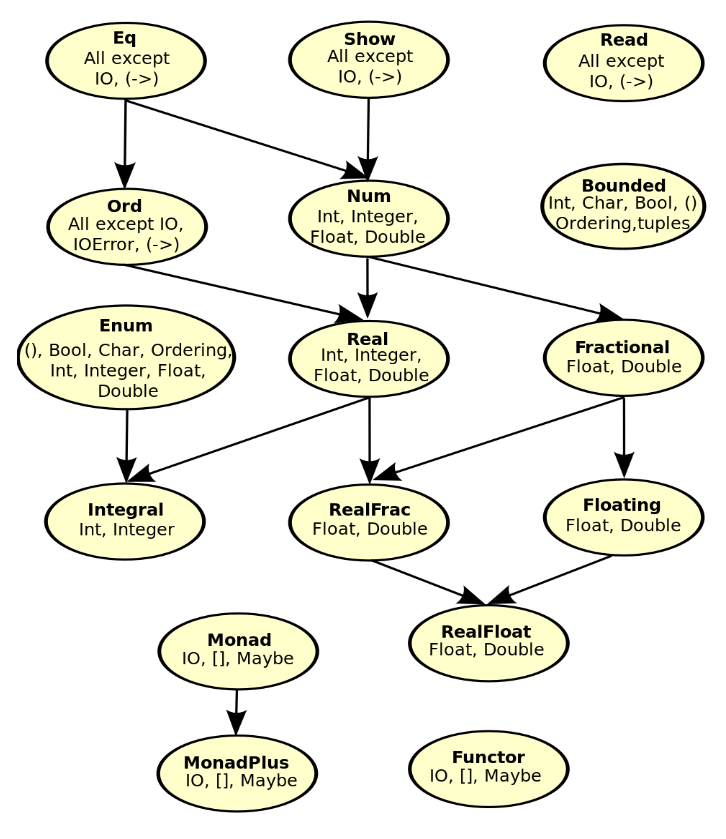
\includegraphics{images/haskell_subclasses.png}
   \caption{Haskell Subclasses relationships}
   \label{fig:haskell_subclasses}
\end{figure}

\end{paracol}

\subsection{Deriving}
For \lstinline|Read|, \lstinline|Show|, \lstinline|Bounded|, \lstinline|Enum|, \lstinline|Eq|, and \lstinline|Ord|, the \ul{compiler can generate instance declarations automatically}.
\begin{lstlisting}
   data Color = Red | Green | Blue
      deriving (Show, Read, Eq, Ord)
   
   Main>:t show
   show :: Show a => a -> String
   Main> show Red
   "Red"
   Main> Red < Green
   True
   Main>:t read
   read :: Read a => String -> a
   Main> let c :: Color = read "Red"
   Main> c
   Red
\end{lstlisting}

\subsection{Numeric Literals}
\begin{lstlisting}
   class Num a where
      (+) :: a -> a -> a
      (-) :: a -> a -> a
      fromInteger :: Integer -> a
      -- Even literals are overloaded.
      -- 1 :: (Num a) => a
      ...

   inc :: Num a => a -> a
   inc x = x + 1
\end{lstlisting}

\labelitemize{
   \textit{Advantages}
}{
   \setlength{\leftskip}{1em}
   Numeric literals can be interpreted as values of any
   appropriate numeric type,
   for example: 1 can be an Integer or a Float or a user-defined numeric type, so it will be interpreted ---for instance--- as \lstinline|fromInteger 1|.
}


\section{Inferencing types}
In standard type checking the compiler examine body of each function and uses declared types to check agreement;
\ul{\textbf{type inference} instead consists in examining code without type information, and infer the
most general types that could have been declared}.

\subsection{Steps schematics}
\begin{figure}[htbp]
   \centering
   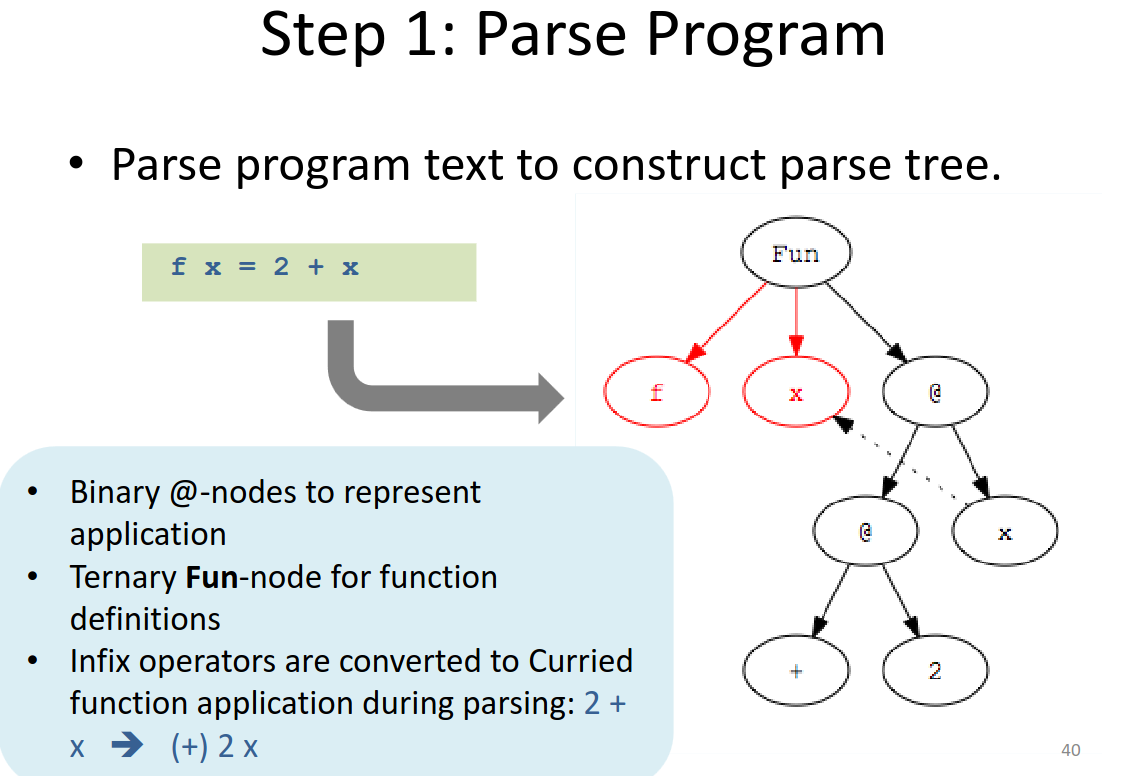
\includegraphics[width=0.4\columnwidth]{images/typeinference_step1.png}
   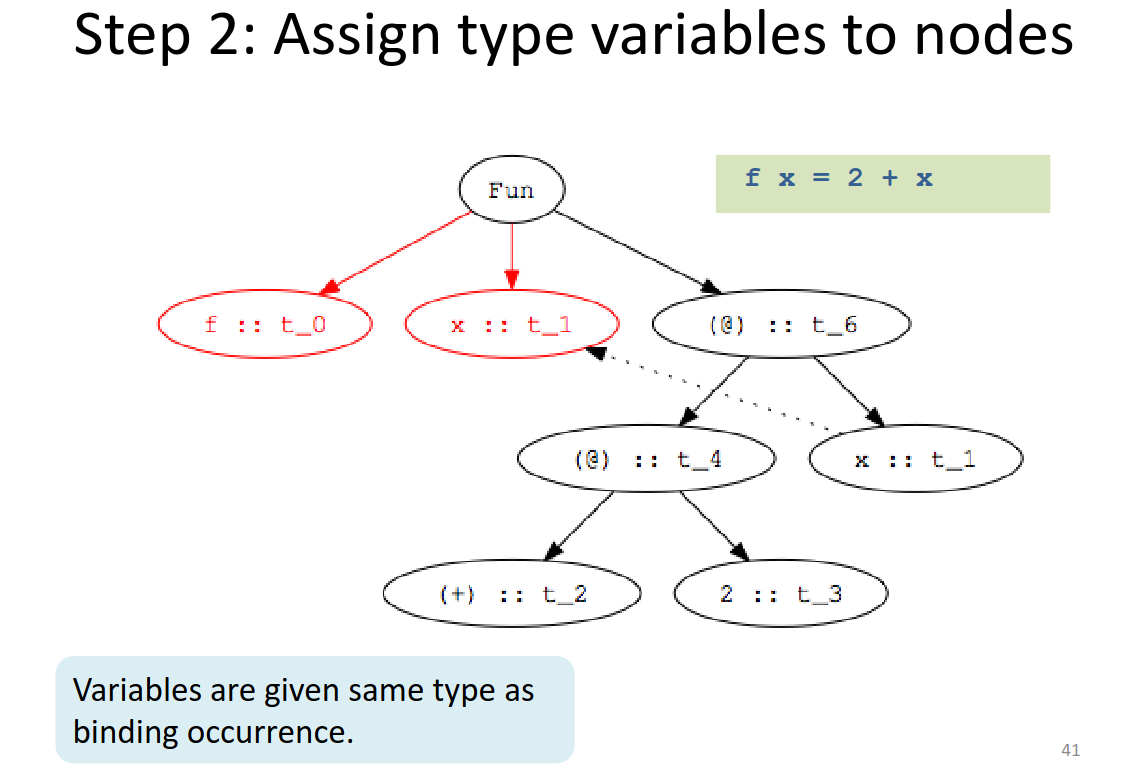
\includegraphics[width=0.4\columnwidth]{images/typeinference_step2.png}
   \label{fig:typeinference_step1_2}
\end{figure}

% \begin{figure}[htbp]
%    \centering
%    \label{fig:typeinference_step2}
% \end{figure}

\textbf{Constraints} can be deduced from (function) \textit{Application} nodes \lstinline|f x| and from \textit{Abstractions} \lstinline|f x = e|.

\begin{figure}[htbp]
   \centering
   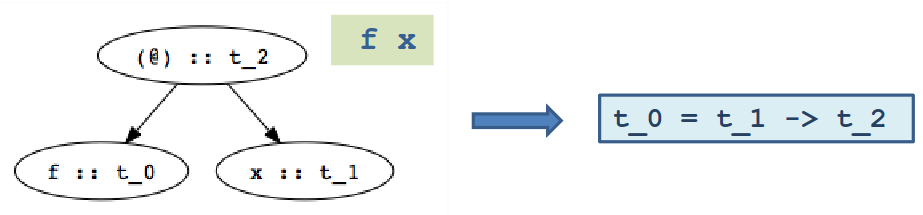
\includegraphics{images/typeinference_constraints_application.png}
   \caption{Deducing constraints from function application}
   \label{fig:typeinference_constraints_application}
\end{figure}
\begin{itemize}
   \item Type of \lstinline|f| (\lstinline|t_0| in figure) must be $domain \longrightarrow range$.
   \item \textbf{Domain} of \lstinline|f| must be type of argument \lstinline|x| (\lstinline|t_1|)
   \item \textbf{Range} of f must be result of application (\lstinline|t_2|)
   \item \textbf{Constraint}: \lstinline|t_0 = t_1 -> t_2|
   \note{\lstinline|LRN| \lstinline|ChildLeft = ChildRight -> Root| }
\end{itemize}

\begin{figure}[htbp]
   \centering
   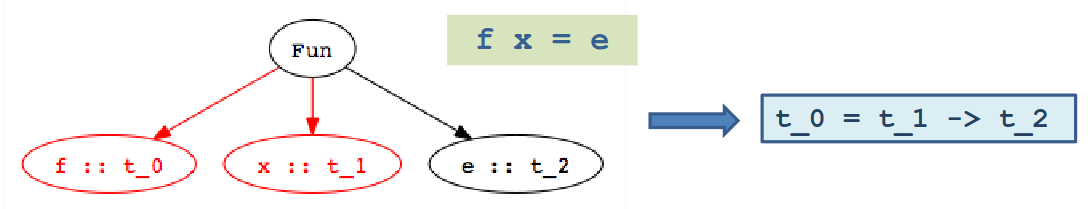
\includegraphics{images/typeinference_constraints_abstraction.png}
   \caption{Deducing constraints from abstractions}
   \label{fig:typeinference_constraints_abstraction}
\end{figure}


\begin{figure}[htbp]
   \centering
   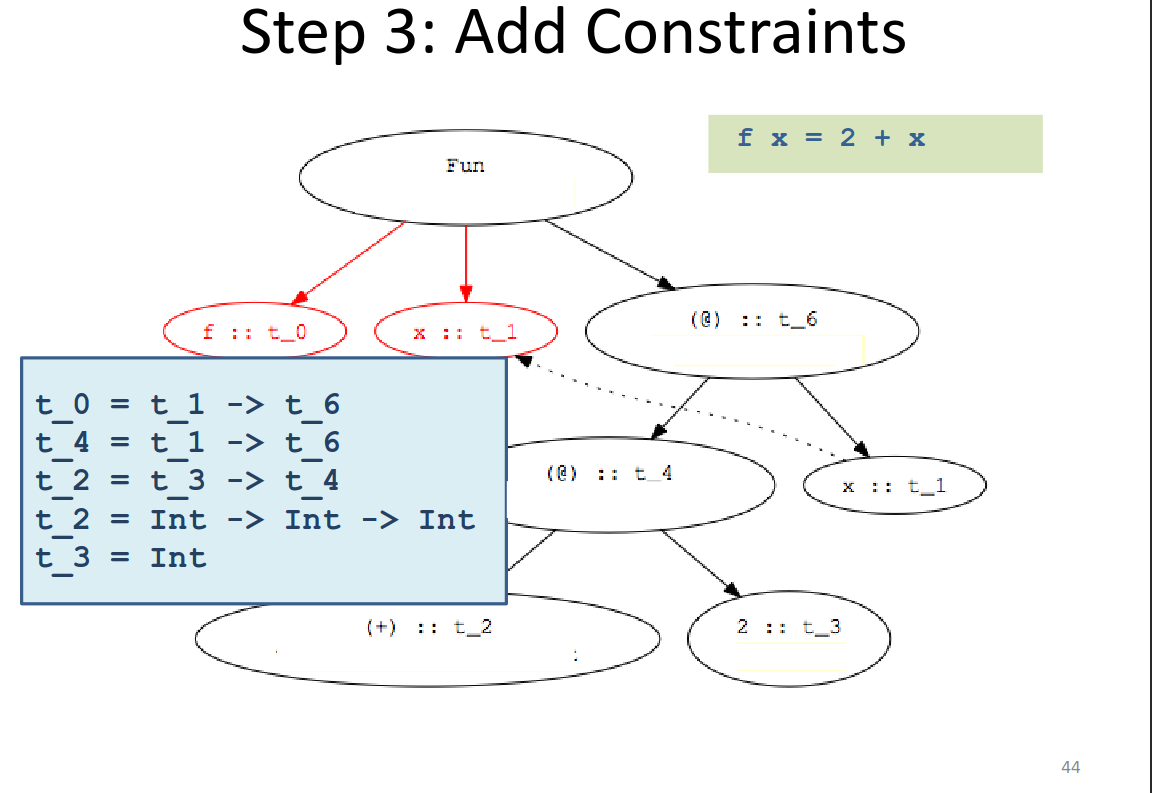
\includegraphics[width=0.4\columnwidth]{images/typeinference_step3.png}
   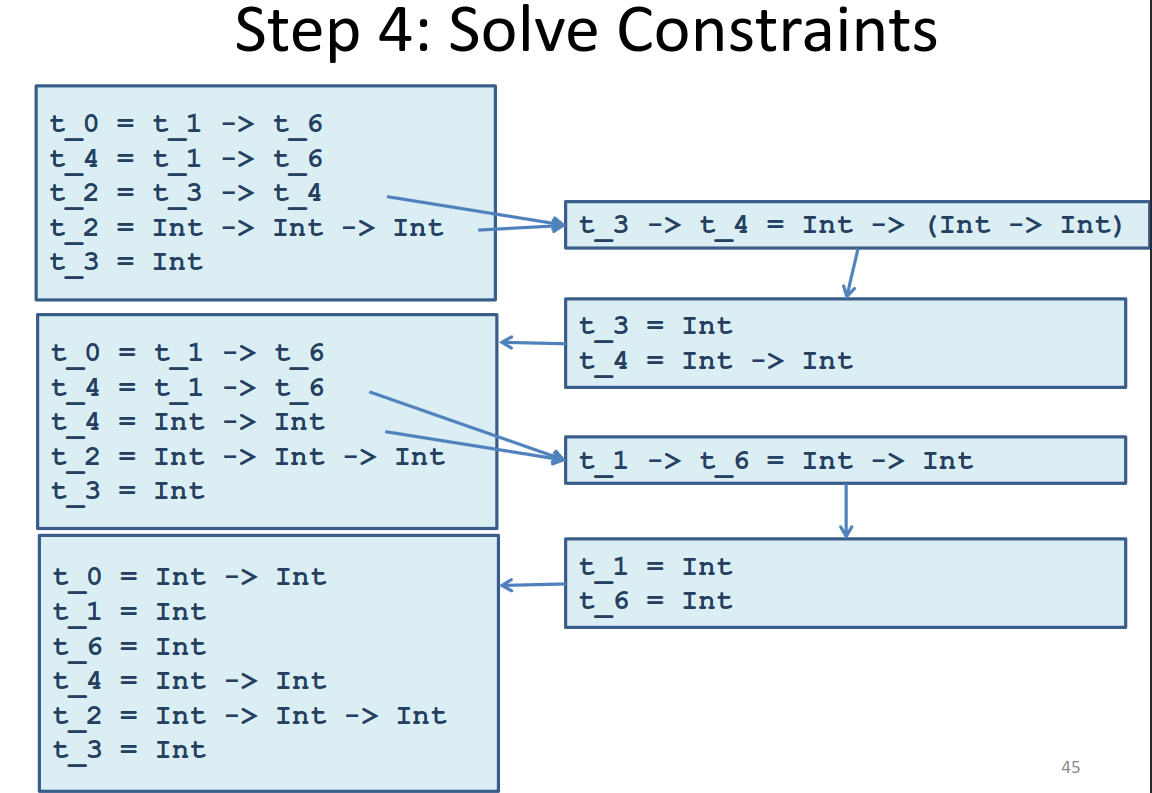
\includegraphics[width=0.4\columnwidth]{images/typeinference_step4.png}
   \label{fig:typeinference_step3_4}
\end{figure}

\begin{figure}[htbp]
   \centering
   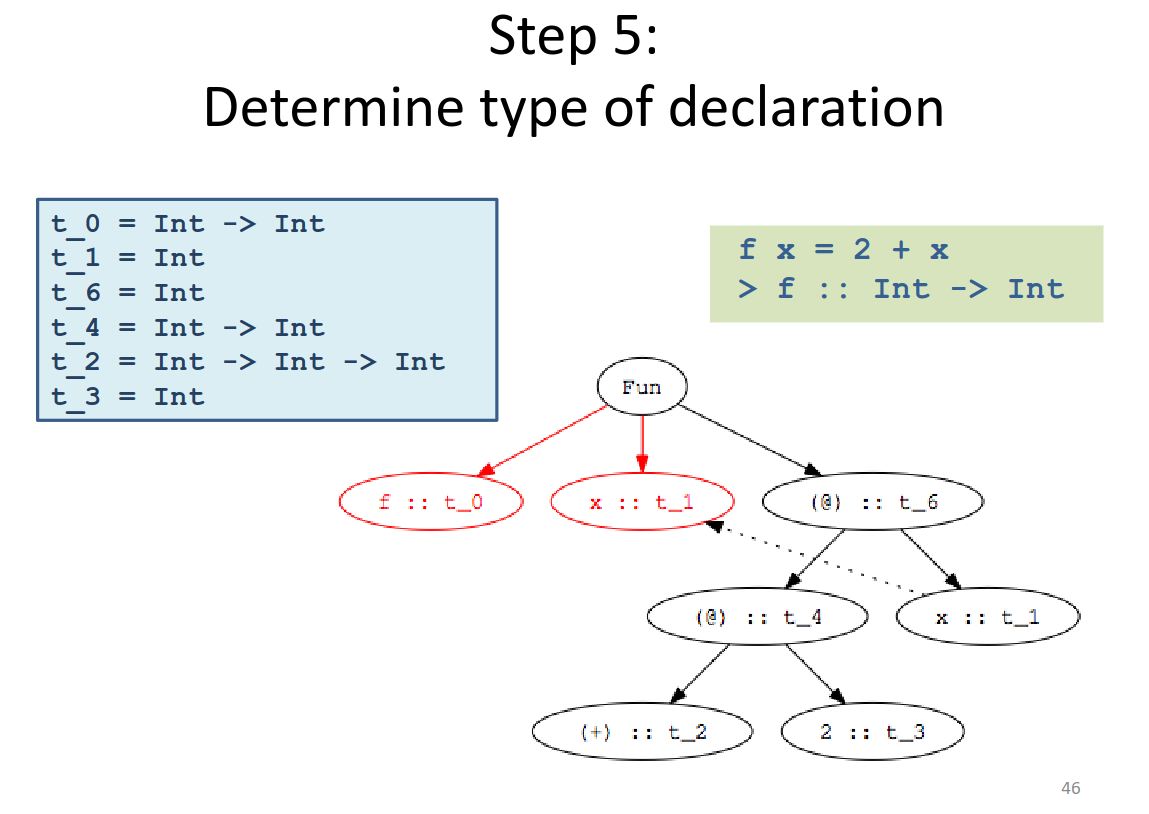
\includegraphics[width=0.4\columnwidth]{images/typeinference_step5.png}
   \label{fig:typeinference_step5}
\end{figure}
\newpage

\subsubsection{Steps summary}
\begin{enumerate}
   \item Parse program to build parse tree
   \begin{itemize}
      \item Each node is a function application \lstinline|@|, variable $x$, or constant
   \end{itemize}
   \item Assign type variables to nodes in tree
   \item Generate constraints:
   \begin{enumerate}
      \item From environment: constants (\lstinline|2|), built-in
      operators (\lstinline|+|), known functions (\lstinline|tail|).
      \item From shape of parse tree: e.g., application and
      abstraction nodes.
   \end{enumerate}
   \item Solve constraints using unification
   \item Determine types of top-level declarations
\end{enumerate}

\subsection{Polymorphism}

In general \textbf{unconstrained} type variables become \textbf{polymorphic types};
for instance, in the example below \lstinline|t_4| is unconstrained, hence we get a polymorphic type:
\begin{lstlisting}
   f g = g 2
   > f :: (Int -> t_4) -> t_4
\end{lstlisting}
\nl

For functions with multiple clauses, i.e. \textit{polymorphic datatypes},
for each clause a separate type is inferred, 
and then the resulting types are combined by adding constraints such as that all clauses have the same type.
In case of \textit{recursive calls}:
the function has same type as its definition.

\begin{lstlisting}
   append ([],r) = r
   append (x:xs, r) = x : append (xs, r)

   -- Actually this could simply be written as xs ++ r
\end{lstlisting}

\begin{enumerate}
   \item Infer type of each clause
   \begin{enumerate}
      \item First clause:
      \begin{lstlisting}
   > append :: ([t_1], t_2) -> t_2
      \end{lstlisting}
      \item Second clause:
      \begin{lstlisting}
   > append :: ([t_3], t_4) -> [t_3]
      \end{lstlisting}
   \end{enumerate}
   \item Combine by equating types of two clauses
   \begin{lstlisting}
   > append :: ([t_1], [t_1]) -> [t_1]
   \end{lstlisting}
\end{enumerate}

\subsection{Overloading}
{In presence of \textbf{overloading} (\textit{Type Classes}), type inference infers a \textbf{qualified type} \lstinline|Q => T|\ns
\begin{itemize}
   \item T is a Hindley Milner type, inferred as seen before
   \item Q is set of type class \textbf{predicates}, called a constraint
\end{itemize}}
\begin{lstlisting}
   example :: Ord a => a -> [a] -> Bool
   example z xs = 
      case xs of
         [] -> False
         (y:ys) -> y > z || (y==z && ys == [z])
\end{lstlisting}

\begin{paracol}{2}
   \colfill
   In the example \textbf{Type} \lstinline|T| is \lstinline|a -> [a] -> Bool|
   while the \textbf{Constraint} \lstinline|Q| is \lstinline|{ Ord a, Eq a, Eq [a]}|.
   \lstinline|Q| later simplifies\footnote{According to some rules not discussed here} to \lstinline|Ord a|
   \colfill
   \switchcolumn

   \begin{itemize}
      \item \lstinline|Ord  a| because \lstinline|y>z|
      \item \lstinline|Eq a| because \lstinline|y==z|
      \item \lstinline|Eq [a]| because \lstinline|ys == [z]|
   \end{itemize}
\end{paracol}

\section{Type Constructors}
\textbf{Type Classes} are \textit{predicates} over \textit{types},
while \textbf{[Type] Constructor Classes} are \textit{predicates} over \textit{type constructors}.
Constructor classes extend the concept of type classes to type constructors. They allow you to specify constraints not just on types but on type constructors as well.

\framedt{About \textit{predicates}}{
   A predicate in logic is a statement or condition that can be true or false, depending on the value it is applied to.\\
   In Haskell, a predicate over types means a constraint or condition on a type, often expressed using a type class. It determines whether a type satisfies some required properties.
}

For example, consider three versions of the \lstinline|map| function (implementation is omitted): the basic one for lists, one for trees and one for \lstinline|Maybe|.
\begin{lstlisting}
   map :: (a -> b) -> [a] -> [b]
   mapTree :: (a -> b) -> Tree a -> Tree b
   mapMaybe :: (a -> b) -> Maybe a -> Maybe b
\end{lstlisting}
They all share the same structure, thus they can all be written as
\begin{lstlisting}
   fmap:: (a -> b) -> g a -> g b
\end{lstlisting}
where \lstinline|g| is a function from \textit{types to types}, i.e.
a \textbf{type constructor};
it is:
\lstinline|[-]| for lists, \lstinline|Tree| for trees, and \lstinline|Maybe| for options.

\subsection{\texttt{Functor}}
This pattern can be captured in a constructor
class \lstinline|Functor|. 
A \textbf{constructor class} is simply a type class where
the predicate is over a type constructor rather
than on a type:
\begin{lstlisting}
   class Functor g where
      fmap :: (a -> b) -> g a -> g b
\end{lstlisting}

Compare with the definition of a \textit{standard type class}:
\begin{lstlisting}
   class Eq a where
      (==) :: a -> a -> Bool
\end{lstlisting}

So, wrapping up, we can instantiate \lstinline|Functor| on all three data structures,
and then simply use the \textit{overloaded} symbol \lstinline|fmap|, instead of \lstinline|map|, \lstinline|mapTree| and \lstinline|mapMaybe|.
\begin{lstlisting}
   class Functor f where
      fmap :: (a -> b) -> f a -> f b
   instance Functor [] where // [] is an instance of Functor
      fmap f [] = []
      fmap f (x:xs) = f x : fmap f xs
   instance Functor Tree where // Tree is an instance of Functor
      fmap f (Leaf x) = Leaf (f x)
      fmap f (Node(t1,t2)) = Node(fmap f t1, fmap f t2)
   instance Functor Maybe where // Maybe is an instance of Functor
      fmap f (Just s) = Just(f s)
      fmap f Nothing = Nothing
\end{lstlisting}

\note{Alternatively we could also write \lstinline|fmap = map|, \lstinline|fmap = mapTree|, fmap = \lstinline|mapMaybe|}

The following is an example on how to use the obtained fmap:
\begin{lstlisting}
   ghci> fmap (\x->x+1) [1,2,3]
   [2,3,4]
   it :: [Integer]
   ghci> fmap (\x->x+1) (Node(Leaf 1, Leaf 2))
   Node (Leaf 2,Leaf 3)
   it :: Tree Integer
   ghci> fmap (\x->x+1) (Just 1)
   Just 2
   it :: Maybe Integer
\end{lstlisting}

\subsection{Comparison with Other Languages}
Type constructors are like functions at the type level; they take type parameters to produce specific types, besides, they also have a \textbf{kind}, which is the type of the type constructor itself (weird right?).
\begin{lstlisting}
   data Maybe a = Nothing | Just a
   data MSet a = MS [(a,Int)]
   data Either a b = Left a | Right b
\end{lstlisting}
\lstinline|Maybe| and \lstinline|MSet| have kind \lstinline|* -> *|, while \lstinline|Either| has kind \lstinline|* -> * -> *|.
Functor for example has kind \lstinline|(* -> *) -> Constraint|, so only type constructors taking one parameter can be instances of \lstinline|Functor|.
However note that \textbf{partial application} works also on type constructors, so \lstinline|Either a| has kind \lstinline|* -> *| and can be an instance of \lstinline|Functor|.
\begin{lstlisting}
   instance Functor (Either e) where
      fmap f (Right x) = Right (f x)
      fmap _ (Left e)  = Left e

   let value = Right 42 :: Either String Int
   fmap (+1) value  -- Result: Right 43

   fmap (++ "!") (Just "hello")           -- Result: Just "hello!"
   fmap (++ "!") (Right "world")          -- Result: Right "world!"
   fmap (++ "!") ["hello", "world"]       -- Result: ["hello!", "world!"]

   -- Concrete type - Fully applied
   type ResultInt = Either String Int

   -- Type constructor - Partially applied (kind * -> *)
   type ResultInt = Either String

\end{lstlisting}

In Java and Scala there is no such thing as partially applying type constructors. For instance, \lstinline|Either<String, T>| in Java or Scala \ul{must always specify both type arguments}. You can't easily abstract over just the second type.\\
Rust behaves similarly, \lstinline|Result<T, E>| (Rust's Either equivalent) requires both types to be specified in full.
Note also that none of these languages have the notion of \textit{kind} of a type constructor. In Java and Scala they implicitly assume kind \lstinline|* -> *|


This architecture allows for \textbf{Higher Kinded Types} (HKT), which are types that take other types as parameters, and are used to define type constructors.
Let's dig in a bit more.

\subsubsection{Java}
Java has no HKT, but it has \textit{Generics}, which are a way to abstract over types. Let's recall down here what \lstinline|fmap| does in Haskell:
\begin{lstlisting}
   a = ["a", "bb", "cccc"]

   b = Just "bb"
   
   main :: IO ()
   main = do
      print $ fmap length a
      print $ fmap length b
\end{lstlisting}
As you can see, \lstinline|fmap| is used to apply a function to the elements of a list or to the value inside a \lstinline|Maybe|, and it works seamlessly for both, since they both are instances of \lstinline|Functor|.

Now, let'see how we could implement \lstinline|fmap| in Java:
\begin{lstlisting}
   public static <C,A,B> C<B> fmap (C<A> a, Function<A,B> f) {
      return f.apply(a);
   }
\end{lstlisting}

This would be cool, but sadly it doesn't compile. \lstinline|C<B>| is absolutely illegal in Java, since Generics lack HKT.
Java cannot understand that \lstinline|C| is a type constructor, and not a concrete type; it doesn't have the notion of kind, so it doesn't know that \lstinline|C| should be applied to a type to produce a type.
There is no difference, at a type level, between \lstinline|List| and \lstinline|List<String>| or \lstinline|Animal| in Java, they are just types.\\
In Java, you can't abstract over type constructors, so you can't define a function that works for both \lstinline|List| and \lstinline|Optional|, for example.

What Java forces us to do is to define a separate \lstinline|fmap| for each type constructor, which is not clean and not DRY ----\textit{Don't Repeat Yourself}--- at all.
\begin{lstlisting}[language=Java]
   public static <A,B> List<B> fmap_list (List<A> a, Function<A,B> f) {
      return a.stream().map(f).collect(Collectors.toList());
   }

   public static <A,B> Set<B> fmap_set (Set<A> a, Function<A,B> f) {
      return a.stream().map(f).collect(Collectors.toSet());
   }
\end{lstlisting}

Besides, a Set cannot be a \lstinline|Functor| not even in Haskell, since applying a function to each element of a Set could possibly change the structure of the Set, which is not allowed for a \lstinline|Functor|.
\begin{lstlisting}
   a = Set [1,2,3,4]
   flatten x = 1
   fmap flatten a = Set [1]
   --- This is not allowed
\end{lstlisting}

\subsubsection{Scala 2}
Scala 2 has HKT, but it's not as powerful as Haskell's.
\begin{lstlisting}[language=Scala]
   trait Functor[F[_]] {
      def fmap[A, B](fa: F[A])(f: A => B): F[B]
    }
    
   object FunctorInstances {
     implicit val listFunctor: Functor[List] = new Functor[List] {
       def fmap[A, B](fa: List[A])(f: A => B): List[B] = fa.map(f)
     }
   
     implicit val optionFunctor: Functor[Option] = new Functor[Option] {
       def fmap[A, B](fa: Option[A])(f: A => B): Option[B] = fa.map(f)
     }
   }
    

   object MyApp extends App {
      // Importing the implicit instances
      import FunctorInstances._
    
      // A generic function that uses the implicit Functor instance
      def transform[F[_], A, B](fa: F[A])(f: A => B)(implicit functor: Functor[F]): F[B] =
        functor.fmap(fa)(f)
    
      // Using the function with Option and List
      val listResult = transform(List(1, 2, 3))((x: Int) => x * 2)  // List(2, 4, 6)
      val optionResult = transform(Option(42))((x: Int) => x + 1)   // Some(43)
    
      println(listResult)
      println(optionResult)
    } 
\end{lstlisting}

\lstinline|F[_]| is a higher-kinded type. It represents any type constructor of kind \lstinline|* -> *|.
fmap works for any type \lstinline|F[_]| as long as there's an instance of \lstinline|Functor[F]| providing the implementation.

\lstinline|implicit| makes these instances available for automatic resolution, so that the compiler finds the appropriate \lstinline|Functor| for the types on which \lstinline|transform| is invoked.
Note that \lstinline|transform| is a generic function that works for any type constructor \lstinline|F[_]| as long as there's an instance of \lstinline|Functor[F]| in scope, it does not care about the specific type constructor, as it happens in Haskell.
Without \lstinline|implicit| we would have to specify the instance explicitly as below, which kills the purpose of this abstraction.
\begin{lstlisting}[language=Scala]
   object OptionFunctor extends Functor[Option] {
     def fmap[A, B](fa: Option[A])(f: A => B): Option[B] = fa.map(f)
   }
   
   val optionExample = OptionFunctor.fmap(Some(42))(_ * 2)   // Some(84
   val listExample = ListFunctor.fmap(List(1, 2, 3))(_ + 1)  // List(2, 3, 4)
\end{lstlisting}

You cannot partially apply type constructors with more than one parameter directly. For example, \lstinline|Either[String, _]| must be written using an alias or type lambda in Scala 2:
\begin{lstlisting}[language=Scala]
   type EitherString[A] = Either[String, A]  // Alias for partial application

   object EitherStringFunctor extends Functor[EitherString] {
     def fmap[A, B](fa: Either[String, A])(f: A => B): Either[String, B] = fa.map(f)
   }
   
\end{lstlisting}

\subsubsection{Rust}
\label{sec:rust_hkt}
Rust does not have HKT, but it has \textit{Traits}, which are similar to type classes in Haskell.
We can mimick to some extent the behavior of \lstinline|Functor| in Rust using Traits, there is an \href{https://hugopeters.me/posts/14/}{article here displaying how}, but is a syntactic mess which I won't report here; below there is only the last part of the code, with the usage of this \lstinline|Functor| trait.
\begin{lstlisting}[language=Rust]
   fn main() {
      let x = Some(5);
      let y = x.fmap(&|i| i+1);
      let z = x.bind(&|_| Applicative::pure(String::from("bound!")));
  
      let x2 : Option<i32>= None;
      let y2 = x2.fmap(&|i| i+1);
      let z2 = x2.bind(&|_| Applicative::pure(String::from("bound!")));
  
      let g: Option<&dyn Fn(&i32) -> String> = Some(&|i| format!("{}={}", i, i));
      let g_eval = <Option<&dyn Fn(&i32) -> String> as Applicative>::ap(&g, &Some(69));
  
      println!("x: {:?}, x2: {:?}, y: {:?}, y2: {:?}, z: {:?}, z2: {:?}, geval: {:?}", x, x2, y, y2, z, z2, g_eval);
  }
\end{lstlisting}

% \lstinline|Inner| represents the type inside the container (e.g., the \lstinline|T| in \lstinline|Option<T>|).
% \lstinline|Output| represents the type of the container after applying the mapping function.
% The fmap function is implemented specifically for \lstinline|Option|, using \lstinline|.map|.

% Rust does not support higher-kinded types, so you cannot write a completely generic \lstinline|fmap| that works for arbitrary type constructors like \lstinline|Option|, \lstinline|Vec|, or \lstinline|Result|. You would need a separate \lstinline|Functor| implementation for each concrete type constructor.
Rust does not support higher-kinded types, however the author of the article claims its solution kinda works like HKT, but still discourages its usage because of the syntactic noise and of the errors and warnings which are arise when using it.

In fact as you can see in the code, \lstinline|fmap| is invoked on the \lstinline|x| instance of \lstinline|Option<i32>|, so it's not generic at all.

